\section{Intro}
\subsection{Introduction}
\frame{%
   \frametitle{\subsecname}
   \framesubtitle{In this presentation}
	\begin{itemize}
	\item Introduction 
	\item Research questions
	\item Sub question
	\item Results 
	\item Conclusion 
	\item Demo
	\end{itemize}
}

\frame{
	\frametitle{\subsecname}
	\framesubtitle{Motive}
	\begin{itemize}
	\item Video game development 
	\item Casanova
	\item Meta Casanova
	\item Front-end of the compiler 
	\end{itemize}
	Meta Casanova became usefull for more then game development
}
\subsection{Research question}
\frame{
	\frametitle{\subsecname}
	\framesubtitle{Main question}
	How to develop a maintainable and expandable front-end and type checker for the Meta Casanova programing language?
}

\frame{
	\frametitle{\subsecname}
	\framesubtitle{Requirements}
	\begin{itemize}
	\item Correct
	\item Maintainable and expandable
	\item Descriptive error messages 
	\end{itemize}
}
\subsection{Sub questions}
\frame{
	\frametitle{\subsecname}
	\begin{itemize}
	\item Syntactic propeties question
	\item Parser question
	\item Type system question
	\end{itemize}
}
\subsection{Syntactic propeties question}
\frame{
	\frametitle{\subsecname}
	What properties does MC have that the front-end needs to process?
	\begin{itemize}
	\item Few keywords
	\item Every definition has a declaration 
	\item Features can be devided in groups
	\end{itemize}
}

\frame{
	\frametitle{\subsecname}
	\framesubtitle{Keywords}
	\begin{multicols*}{2}
	MC
	\begin{itemize}
	\item Func
	\item Data
	\item TypeFunc
	\item TypeAlias
	\item ->
	\item =>
	\item \#>
	\item import
	\item inherit
	\item Module
	\item (\textbackslash  ...code...  )
	\end{itemize}
	\columnbreak
	C\#

	abstract ; as ; base ; bool ;
    break ; byte ; case ; catch ; char ; checked ; class ; const ;
    continue ; decimal ; default ; delegate ; do ; double ; else ;
    enum ; event ; explicit ; extern ; false ; finally ; fixed ; 
    float ; for ; foreach ; goto ; if ; implicit ; in ; int ; 
    interface ; internal ; is ; lock ; long ; namespace ; new ;
    null ; object ; operator ; out ; override ; params ; private ;
    protected ; public ; readonly ; ref ; return ; sbyte ; sealed ;
    short ; sizeof ; stackalloc ; static ; string ; struct ; 
    switch ; this ; throw ; true ; try ; typeof ; uint ; ulong ; 
    unchecked ; unsafe ; ushort ; using ; virtual ; void ; 
    volatile ; while
    \end{multicols*}
}

\frame{
	\frametitle{\subsecname}
	\framesubtitle{Devided features}
	\begin{itemize}
	\item Data and func
	\item Dotnet
	\item lambdas
	\item TypeAlias
	\item TypeFunc
	\item Module
	\end{itemize}

}
\subsection{Parser question}
\frame{
	\frametitle{\subsecname}
	How to develop a maintainable and expandable parser for MC?
}

\frame{
	\frametitle{\subsecname}
	\framesubtitle{What is a parser}
	\begin{itemize}
	\item Takes a sequence of elements
	\item Builds a data structure
	\item Detect syntactic errors
	\end{itemize}
}

\frame{
	\frametitle{\subsecname}
	\framesubtitle{How to make a parser}
	\begin{itemize}
	\item Parser generators
	\item Parser monad
	\end{itemize}
}

\frame{
	\frametitle{\subsecname}
	\framesubtitle{Parser generator}
	\begin{itemize}
	\item Is a program
	\item Syntax description -> parser
	\end{itemize}
}
\frame{
	\frametitle{\subsecname}
	\framesubtitle{Parser generator}
	\begin{multicols*}{2}
	Pros 
	\begin{itemize}
	\item Fast setup
	\item Fast parsing
	\end{itemize}
	\columnbreak
	Cons
	\begin{itemize}
	\item Difficult to generate helpful error messages
	\end{itemize}
	\end{multicols*}
}

\frame{
	\frametitle{\subsecname}
    \framesubtitle{What is a parser monad?}
    A parser monad iterates over a list and builds a output structure.

    If the parser fails then instead of the context it will return an error.
}

\frame{
    \frametitle{\subsecname}
    \framesubtitle{concat}
    \begin{multicols*}{3}
    \begin{enumerate}
    \item t \item w \item o \item \# \item w \item o \item r \item d \item s \item \#
    \end{enumerate}
    \columnbreak
    ch = get-char
    concat ch
    \columnbreak
    \begin{enumerate}
    \item two\#words\#
    \end{enumerate}
    \end{multicols*}
}
\frame{
    \frametitle{\subsecname}
    \framesubtitle{check char}
    \begin{multicols*}{3}
    \begin{enumerate}
    \item t \item w \item o \item \# \item w \item o \item r \item d \item s \item \#
    \end{enumerate}
    \columnbreak
    check-char \#
    \columnbreak
    \begin{enumerate}
    \item nope \item nope \item nope \item yep \item nope \item nope \item nope \item nope \item nope \item yep
    \end{enumerate}
    \end{multicols*}
}
\frame{
    \frametitle{\subsecname}
    \framesubtitle{until}
    \begin{multicols*}{3}
    \begin{enumerate}
    \item t \item w \item o \item \# \item w \item o \item r \item d \item s \item \#
    \end{enumerate}
    \columnbreak
    ch = get-char until check-char \#

    concat ch
    \columnbreak
    \begin{enumerate}
    \item two \item words
    \end{enumerate}
    \end{multicols*}
}

\frame{
    \frametitle{\subsecname}
    \framesubtitle{Error handling within the parser monad}
    \begin{multicols*}{3}

    Concat all the errors
    \begin{enumerate}
    \item Slow
    \item Get all the errors and thus none
    \end{enumerate}

    \columnbreak

    Give only the last viable error
    \begin{enumerate}
    \item Fast
    \item possibility to lose error information
    \item possibility to get incorrect error information
    \end{enumerate}

    \columnbreak

    Priority for errors
    \begin{enumerate}
    \item Fast
    \item More accurate error information
    \item possibility to get incorrect error information
    \end{enumerate}
    \end{multicols*}
}

\frame{
    \frametitle{\subsecname}
    \framesubtitle{Errors with priority}
    The error with the highest priority is the one that gets returned.
    \begin{figure}
        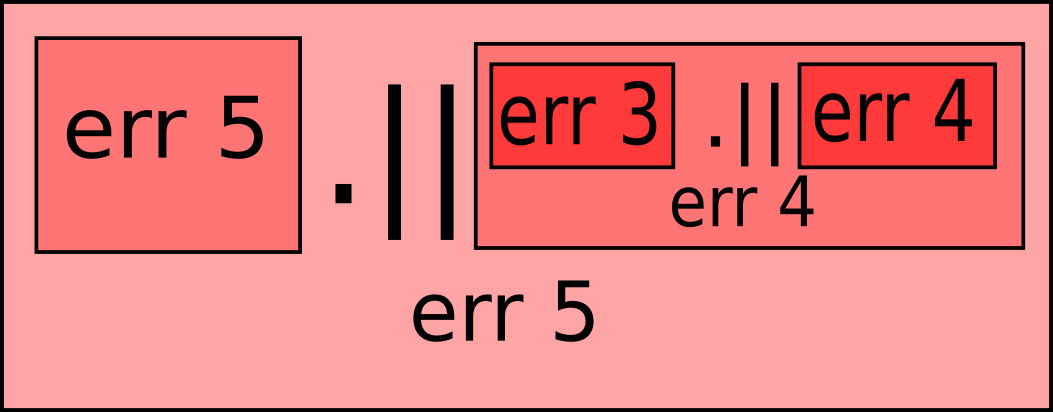
\includegraphics{error_example}
    \end{figure}
}
\frame{
    \frametitle{\subsecname}
    \framesubtitle{parser monad}
    \begin{multicols*}{2}
    Pros 
    \begin{itemize}
	\item Custom error system
	\item Powerful parser
	\item Easy to maintain and expand	
	\end{itemize}
	\columnbreak
	Cons
	\begin{itemize}
	\item Slow setup
	\item Slow parsing
	\end{itemize}
    \end{multicols*}
}

\frame{
    \frametitle{\subsecname}
    \framesubtitle{Strategy}
    \begin{multicols*}{2}
    \begin{itemize}
	\item Data and func
	\item Dotnet
	\item lambdas
	\item TypeAlias
	\item TypeFunc
	\item Module
	\end{itemize}
	\columnbreak
	\begin{itemize}
	\item Minimal type checker    
	\item DotNet types 
	\item Type inference 
	\item Kind support 
	\item Compile time interpretation    
	\item Complex inheritance system 
	\end{itemize}
	\end{multicols*}
}

\frame{
    \frametitle{\subsecname}
    \framesubtitle{Modules}
    \begin{itemize}
	\item Declarations TypeFunc and Alias
	\item Definitions TypeFunc and Alias
	\item Declarations Data and Function
	\item Definitions Rules    
	\end{itemize}
}
\subsection{Type system question}
\frame{
    \frametitle{\subsecname}
    How to apply type systems to MC?
}

\frame{
    \frametitle{\subsecname}
    \framesubtitle{Type checker}
    \begin{itemize}
	\item Normalized input and output
	\item Modular
	\item Separate type checker for run-time and compile time components  
	\end{itemize}
}

\frame{
    \frametitle{\subsecname}
    \framesubtitle{Normalization}
    \begin{itemize}
	\item Smaller type checker
	\item Less complexity in data structures  
	\end{itemize}
}

\frame{
    \frametitle{\subsecname}
    \framesubtitle{Modular}
    Just like the parser
    \begin{itemize}
	\item Declarations TypeFunc and Alias
	\item Definitions TypeFunc and Alias
	\item Declarations Data and Function
	\item Definitions Rules    
	\end{itemize}
}

\frame{
    \frametitle{\subsecname}
    \framesubtitle{Separate type checker for run-time and compile time components}
    \begin{itemize}
	\item Helps getting the first prototype working faster
	\item Extra securety on type checking
	\end{itemize}
}

\subsection{Detour with the customer}

\frame{
    \frametitle{\subsecname}
    \begin{itemize}
	\item Request for full Mark 3 compiler
	\item Will take longer then I have time for
	\item Customer wants to make a type checker for it
	\item His type checker is not compatible with the current compiler
	\item Solution: I make a parser for the customer his type checker
	\end{itemize}
}

\subsection{Conclusion}

\frame{
    \frametitle{\subsecname}
    \begin{itemize}
    \item A parser has been made to process the features of MC
    \item The parser can give descriptive error messages
    \item The front-end is designed to be maintainable and expandable
    \item A type checker was created for the run time features of MC
    \end{itemize}
}

\subsection{Demo}

\frame{
    \frametitle{\subsecname}
    The front-end generates a correct data structure for the back-end
}

\subsection{Questions}

\frame{
    \frametitle{\subsecname}

}